\documentclass[tikz,border=0cm,dvipsnames,x11names,rgb]{standalone}

\usepackage{amsmath,amssymb,amsfonts}
\usetikzlibrary{calc,
fit,
shapes.misc,
shapes.geometric,
arrows.meta,
fadings,
matrix,
chains,
scopes,
positioning}

\usepackage{pgfplots}
\usepackage{pgfplotstable}
\pgfplotsset{compat=1.18}



\usepackage[]{fontspec}

\setmainfont{Latin Modern Roman}
\setmonofont{Latin Modern Math}
\renewcommand{\textsc}[1]{{\fontfamily{lmr}\selectfont \scshape #1}}

\usepackage[]{bm}

\makeatletter
\@ifundefined{fromRoot}{\newcommand{\fromRoot}[1]{../../#1}}{}

\def\input@path{{../..}{..}{.}{./svg}{./pgfplots}{./tikzpicture}}
%or: \def\input@path{{/path/to/folder/}{/path/to/other/folder/}}
\makeatother

\newcommand{\ra}[1]{\renewcommand{\arraystretch}{#1}}

\newcommand*{\gf}[1]{\acrshort{gf}($#1$)}%
\newcommand*{\mpn}[1]{\bm{P}_{#1}}%
\newcommand*{\pn}[1]{%
  \ifthenelse{\equal{#1}{}}{$\mpn{0}$}{$\mpn{#1}$}%
}%

\newcommand*{\pk}[3]{%
  \ifthenelse{\equal{#1}{#2}}{\textcolor{red}{\phantom{.}$p_0$\phantom{.}}}{\phantom{.}$p_#3$\phantom{.}}%
}%


\newcommand*{\placeholderreg}{\includegraphics[width=\linewidth, height=.25\textheight, keepaspectratio = true]{figures/certified_xilinx.png}}%
\newcommand*{\placeholder}[1]{\includegraphics[#1]{figures/certified_xilinx.png}}%

\newcommand*{\snr}{\acrshort{snr}}%
\newcommand*{\snrs}{\acrshortpl{snr}}%

\newcommand*{\mpd}[0]{p_\Delta}%
\newcommand*{\mpo}[0]{p_\omega}%
\newcommand*{\pd}[0]{$\mpd$}%
\newcommand*{\po}[0]{$\mpo$}%
\newcommand*{\mpfa}[0]{\mathcal{P}_{fa}}%
\newcommand*{\mpmd}[0]{\mathcal{P}_{md}}%
\newcommand*{\pfa}[0]{\acrshort{pfa}}%
\newcommand*{\pmd}[0]{\acrshort{pmd}}%
\newcommand*{\mnorm}[1]{\mathcal{L}_{#1}}%
\newcommand*{\norm}[1]{$\mnorm{#1}$}%
\newcommand*{\fft}{\acrshort{fft}}%
\newcommand*{\mfft}[1]{\mathcal{F}(#1)}%
\newcommand*{\mifft}[1]{\mathcal{F}^{-1}(#1)}%
\newcommand*{\ts}{\acrshort{ts}}%

\newcommand*{\cpp}[1]{C\textrm{++#1}}%
\newcommand*{\na}{\textrm{\textcolor{SlateGray4}{N/A}}}%

\newcommand*{\vect}[1]{\bm{#1}}%
\newcommand*{\mat}[1]{\bm{\mathrm{#1}}}%

\newcommand*{\task}[1]{\mathcal{T}_{#1}}%

\newcommand*{\sdr}{\acrshort{sdr}}%
\newcommand*{\fpga}{\acrshort{fpga}}%

\newcommand*{\rikiki}{\fontsize{4}{6}\selectfont}%


\begin{document}
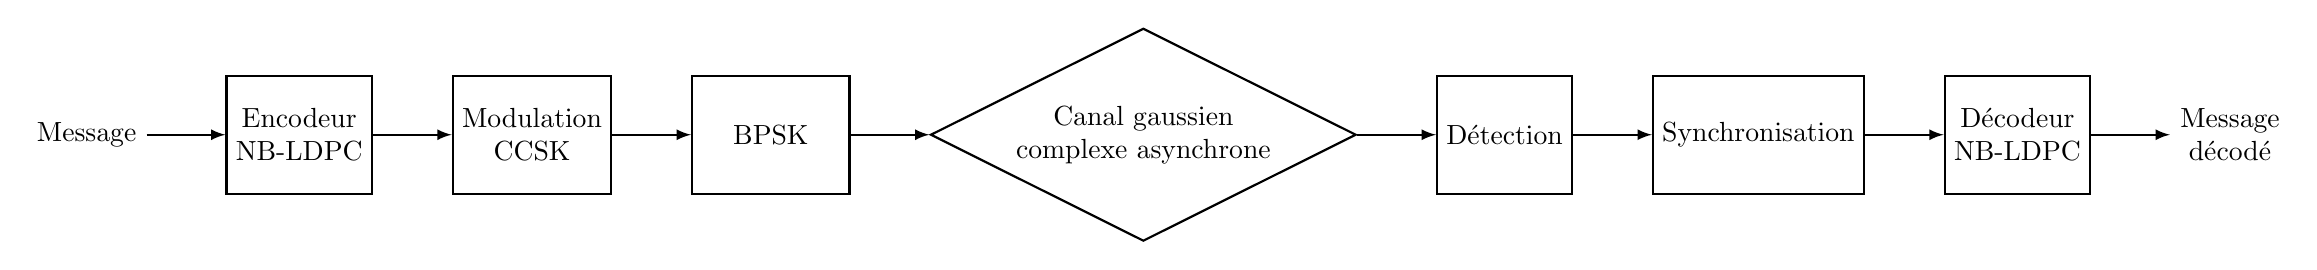
\begin{tikzpicture} [-latex,
    >=latex,
    auto,
    thick,
    main node/.style={rectangle, fill = white!35, draw,
        align=center}
  ]

  \node [main node,
    align=center,
    minimum height = 1.5cm
  ] (nbenc) at (0, 0) {Encodeur\\NB-LDPC};

  \node [main node,
    minimum height = 1.5cm,
    right = 1cm of nbenc
  ] (ccskm) {Modulation\\CCSK};

  \node [main node,
    minimum height = 1.5cm,
    minimum width = 2cm,
    right = 1cm of ccskm
  ] (bpskm) {BPSK};% $+$\\Surmodulation};

  \node [diamond,
    aspect = 2,
    draw,
    fill = white,
    align = center,
    right = 1cm of bpskm,
  ] (bichan)  {Canal gaussien\\complexe asynchrone};

  \node [main node,
    minimum height = 1.5cm,
    %minimum width = 3cm,
    right = 1 cm of bichan
  ] (ccskd)  {Détection};

  \node [main node,
    minimum height = 1.5cm,
    %minimum width = 3cm,
    right = 1 cm of ccskd
  ] (ccsks) {Synchronisation};

  \node [main node,
    minimum height = 1.5cm,
    right = 1cm of ccsks
  ] (nbdec) {Décodeur\\NB-LDPC};

  %%%%%%%%%%%%%%%%%%%%%%%%%%%%%%

  \draw ($(-1, 0) + (nbenc.west)$) -> (nbenc.west)
  node [pos=0, align=center, left] (M) {Message};
  \draw (nbenc.east) -> (ccskm.west);
  \draw (ccskm.east) -> (bpskm.west);
  \draw (bpskm.east) -- (bichan.west);
  \draw (bichan.east) -- (ccskd.west);
  \draw (ccskd.east) -> (ccsks.west);
  \draw (ccsks.east) -> (nbdec.west);
  \draw (nbdec.east) -> ($(1, 0) + (nbdec.east)$)
  node [pos=1, align=center, right] (M) {Message\\décodé};


\end{tikzpicture}
\end{document}
